\chapter{Sistema de detección de emociones}
\label{cap:capitulo4}

En este capítulo se describe el sistema de detección de emociones desarrollado en este trabajo, así como su integración en ROS. Además, se muestra su funcionamiento y rendimiento final.\\

Existen múltiples técnicas utilizadas para realizar detección de emociones, en el artículo \cite{literature_review} encontramos una revisión del estado del arte de los últimos años. En este trabajo, se ha escogido la técnica comprendida por los siguientes tres pasos: detección de puntos faciales, extracción de información de esos puntos faciales, clasificación de esa información. En la Figura \ref{fig:metodo} se muestra un esquema general del funcionamiento del sistema, obviando la integración en ROS, la cual se describe en la Sección \ref{sec:integración_en_ros}. Cada una de las fases de desarrollo mostradas en dicho esquema se corresponde a una sección de este capítulo.\\

\begin{figure} [h!]
  \begin{center}
    \includegraphics[width=16cm]{figs/metodo.png}
  \end{center}
  \captionsetup{justification=centering}
  \caption{Método de detección de emociones.}
  \label{fig:metodo}
\end{figure}

Cabe añadir que el motivo de elegir la técnica descrita anteriormente es debido a que es un método con bajo coste computacional y además es de los más precisos, algo esencial para aportar robustez a la herramienta robótica final de este trabajo.

\section{Detección de puntos faciales}
\label{sec:deteccion_de puntos}

El primer paso del método escogido en este trabajo consiste en realizar una detección de puntos faciales característicos. En búsqueda de la máxima optimización, se hizo un estudio comparando dos librerías de extracción de puntos faciales para obtener conclusiones de cual nos ofrecía más rendimiento y precisión. Estas dos librerías son dlib y MediaPipe, ya presentadas en las secciones \ref{sec:dlib} y \ref{sec:mediapipe}, escogidas por ser las más usadas dentro de la investigación de este campo en publicaciones como, por ejemplo, los artículos \cite{dlib_emotions} o \cite{mediapipe_emotions}. Este estudio y sus resultados se describen detalladamente en la Sección \ref{sec:estudio_puntos_faciales}.\\

El algoritmo que mejores resultados obtuvo fue MediaPipe FaceMesh, obteniendo un rendimiento de 13.28 fps de media y es, por lo tanto, el usado en este sistema. Este algoritmo nos brinda información de coordenadas 3D de 468 puntos faciales (Figura \ref{fig:mediapipe_malla}).\\

\begin{figure} [h!]
  \begin{center}
    \includegraphics[width=9cm]{figs/canonical_face_model_uv_visualization.png}
  \end{center}
  \captionsetup{justification=centering}
  \caption{Malla facial de MediaPipe de 468 puntos.}
  \label{fig:mediapipe_malla}
\end{figure}

\section{Extracción de información de los puntos faciales}
\label{sec:extraer_informacion}

Tras obtener datos en coordenadas de los puntos faciales característicos de un rostro, debemos tratarlos para que a partir de ellos obtengamos información de las posibles emociones que en ese momento se estén llevando a cabo en el rostro estudiado y, finalmente, crear un dataset con toda esa información que nos permita entrenar modelos de la forma más precisa posible.\\

Retomando la extracción de información, uno de los métodos más usados hasta ahora es la utilización de las distancias entre puntos faciales, tal como se realiza en el artículo \cite{dlib_emotions} (Figura \ref{fig:dlib_foto_articulo}). Por ejemplo, una emoción de \textit{sorpresa} estará caracterizada por poseer grandes distancias entre el labio inferior y la nariz (boca abierta). Sin embargo, esta técnica es propensa a confundir unas emociones con otras, la información de distancias no es suficiente en determinados casos, ya que a veces se puede mantener constante aunque la expresión facial haya cambiado.

\begin{figure} [h!]
  \begin{center}
    \includegraphics[width=7cm]{figs/dlib_foto_articulo.png}
  \end{center}
  \captionsetup{justification=centering}
  \caption{Distancias entre puntos faciales del artículo \cite{dlib_emotions}.}
  \label{fig:dlib_foto_articulo}
\end{figure}

El método usado para extraer información de los puntos faciales, por lo tanto, no será el relatado anteriormente, sino que se usará un novedoso método propuesto en el artículo \cite{mediapipe_emotions}. Este consiste en construir una \textit{malla emocional} (Figura \ref{fig:malla_emocional}), basada en el Sistema de Codificación Facial o FACS (Facial Action Coding System)\cite{Ekman1978FacialAC}\cite{Ekman1978FacialACManual}, que nos proporcionará información en ángulos de las expresiones faciales.

\begin{figure} [h!]
  \begin{center}
    \includegraphics[width=13cm]{figs/emotional_mesh.png}
  \end{center}
  \captionsetup{justification=centering}
  \caption{\textit{Malla emocional} propuesta en el artículo \cite{mediapipe_emotions}.}
  \label{fig:malla_emocional}
\end{figure}

FACS es un sistema que clasifica movimientos faciales humanos basándose en los cambios producidos en la cara a cargo de los movimientos de los músculos. Estos movimientos son definidos como Unidades de Acción o AUs (Action Units), de los cuales existen hasta 46. En el Cuadro \ref{cuadro:au}, están expuestas las AUs más usadas con sus respectivas descripciones.\\

Por otro lado, el sistema EMFACS (Emotional Facial Action Coding System) describe emociones simples usando combinaciones de AUs (Cuadro \ref{cuadro:emfacs}). Por lo tanto, sabiendo esto, se puede afirmar que el movimiento de cada uno de esos músculos faciales está relacionado con siete emociones simples, y es por eso que cada ubicación de los puntos de la \textit{malla emocional} (Figura \ref{fig:malla_emocional}) ha sido elegida de manera que se vea afectada por una AU y de esta manera conseguir un mejor reconocimiento de emociones.\\

\begin{table}[H]
\begin{center}
\begin{tabular}{|c|c|}
     \hline
    \textbf{AU} & \textbf{Descripciones FACS} \\
    \hline
     1 & Interior de las cejas elevado\\ 
     2 & Exterior de las cejas elevado \\ 
     4 & Cejas bajadas \\
     5 & Párpado superior elevado\\
     6 & Mejillas elevadas \\ 
     7 & Párpados tensos \\
     9 & Nariz arrugada \\
     10 & Labio superior elevado \\
     12 & Comisuras de los labios elevados \\ 
     15 & Comisuras de los labios hacia abajo \\
     16 & Labio inferior hacia abajo \\
     17 & Barbilla elevada \\
     20 & Labios apretados y estirados\\
     22 & Labios en forma de \textit{o} \\
     23 & Labios tensos \\
     24 & Labios presionados \\
     25 & Labios separados \\
     26 & Boca abierta (mandíbula caída)\\
     27 & Boca abierta \\
     \hline
 \end{tabular}
 \captionsetup{justification=centering}
\caption{Lista de las Unidades de Acción más usadas y sus respectivas descripciones FACS.}
\label{cuadro:au}
\end{center}
\end{table}

\begin{table}[H]
\begin{center}
\begin{tabular}{|c|c|}
     \hline
    \textbf{Emoción} & \textbf{AU} \\
    \hline
     Felicidad & 6 + 12\\ 
     Tristeza & 1 + 4 + 15 \\ 
     Sorpresa & 1 + 2 + 5 + 26 \\
     Miedo & 1 + 2 + 4 + 5 + 7 + 20 + 26\\
     Enfado & 4 + 5 + 7 + 23 \\ 
     Asco & 9 + 15 + 17 \\
     Desprecio & 12 + 14 \\
     \hline
 \end{tabular}
 \captionsetup{justification=centering}
\caption{Lista de emociones simples en términos de AUs.}
\label{cuadro:emfacs}
\end{center}
\end{table}

Cada uno de los puntos de la \textit{malla emocional} está unido a otros mediante aristas, formando así una malla cerrada de 27 vértices y 38 aristas. Estas aristas forman ángulos entre ellas, y serán estos los utilizados como información para clasificar emociones. Aprovechando que todas las aristas forman triángulos entre sí (Figura \ref{fig:triangulo}), para calcular los ángulos deseados se utilizará el teorema del coseno (Ecuación \ref{ec:teorema_coseno}), el cual usa la longitud de las aristas para realizar los cálculos, esto es la distancia entre los dos puntos que conforman la arista. Esta distancia es calculada mediante distancia euclídea (Ecuación \ref{ec:ecuclidea_puntos}). En forma de código de Python, las funciones que realizarán esta tarea se encuentran en el Código \ref{cod:angulos}.

\begin{figure} [h!]
  \begin{center}
    \includegraphics[width=5cm]{figs/triangulo.png}
  \end{center}
  \captionsetup{justification=centering}
  \caption{Ejemplo de triángulo formado por 2 aristas de la \textit{malla emocional}.}
  \label{fig:triangulo}
\end{figure}

\begin{myequation}[h]
\begin{equation}
\alpha = \arccos{\frac{l_{1}^{2}+l_{3}^{2}-l_{2}^{2}}{2l_{1}l_{3}}}
\nonumber
\label{ec:teorema_coseno}
\end{equation}
\captionsetup{justification=centering}
\caption[Teorema del coseno para calcular el ángulo de la Figura \ref{fig:triangulo}.]{Teorema del coseno para calcular el ángulo de la Figura \ref{fig:triangulo}.}
\end{myequation} 

\begin{myequation}[h]
\begin{equation}
l_{3} = \sqrt{(p_{1x}-p_{2x})^{2}+(p_{1y}-p_{2y})^{2}}
\nonumber
\label{ec:ecuclidea_puntos}
\end{equation}
\captionsetup{justification=centering}
\caption[Distancia euclídea entre los puntos $p_{1}$ y $p_{2}$ de la Figura \ref{fig:triangulo}.]{Distancia euclídea entre los puntos $p_{1}$ y $p_{2}$ de la Figura \ref{fig:triangulo}.}
\end{myequation} 

\begin{code}[h]
\begin{lstlisting}[style=Python]
def distance(self, point1, point2):
    x0 = point1[0]
    y0 = point1[1]
    x1 = point2[0]
    y1 = point2[1]
    return math.sqrt((x0 - x1)**2+(y0 - y1)**2)

def angle(self, point1, point2, point3):
    side1 = self.distance(point2, point3)
    side2 = self.distance(point1, point3)
    side3 = self.distance(point1, point2)
    
    angle = math.degrees(math.acos((side1**2+side3**2-side2**2)/(2*side1*side3)))
    return angle
\end{lstlisting}
\captionsetup{justification=centering}
\caption[Funciones de Python para realizar el cálculo de ángulos\\
de la \textit{malla emocional}.]{Funciones de Python para realizar el cálculo de ángulos\\
de la \textit{malla emocional}.}
\label{cod:angulos}
\end{code}

\section{Generación del dataset}
\label{sec:generacion_dataset}

Siguiendo el esquema de la Figura \ref{fig:metodo}, el paso siguiente a la extracción de información de los puntos faciales es la generación de un dataset (base de datos) con dicha información, para posteriormente entrenar un modelo usando técnicas de Machine Learning y que este nos permita clasificar emociones. Poseer un buen conjunto de datos es la fase más importante del trabajo; existen proyectos muy buenos que han llegado a fracasar por no poseer un buen dataset. Por lo tanto, hay que dedicar gran parte del tiempo total a la construcción del mismo. Es importante que contenga una buena cantidad de datos y que estos aporten generalidad.\\

La idea llevada a cabo en este trabajo ha sido, en primer lugar, localizar un dataset de imágenes que contenga emociones de distintos sujetos. Seguidamente, tratar cada una de esas imágenes con la \textit{malla emocional} y extraer ángulos de cada una de las emociones. Por último, con esos ángulos, generar un nuevo dataset, que ya nos sirve para entrenar nuestros modelos. En dicho dataset final, el número de muestras es el número de fotografías del primer dataset, y el número de características de cada muestra es la cantidad de ángulos usados de la \textit{malla emocional}.\\

En cuanto al dataset de imágenes, tras realizar una búsqueda por conseguir las imágenes que mejor se adaptasen a nuestro método, se decidió usar \textit{The Extended Cohn-Kanade Dataset (CK+)}\cite{Kanade1}\cite{Kanade2} (Figura \ref{fig:ejemplosCK}). \\

\begin{figure}[h!]
  \begin{center}
    \subcapcentertrue
    \subfigure[Sujeto triste]{\includegraphics[width=50mm]{figs/sujeto_triste.png}}
    \subfigure[Sujeto feliz]{\includegraphics[width=50mm]{figs/sujeto_feliz.png}}
    \subfigure[Sujeto sorprendido]{\includegraphics[width=50mm]{figs/sujeto_sorprendido.png}}
  \end{center}
\captionsetup{justification=centering}
\caption{Ejemplos de imágenes del dataset \textit{The Extended Cohn-Kanade Dataset (CK+)}.}
\label{fig:ejemplosCK}
\end{figure}

Esta base de datos contiene 593 secuencias de imágenes, en las que se muestra un rostro desde una posición neutral hasta la máxima expresión. De esas 593 secuencias, 327 poseen el último \textit{frame} etiquetado con una emoción entre 1 y 7 (1 = anger, 2 = contempt, 3 = disgust, 4 = fear, 5 = happy, 6 = sadness, 7 = surprise). Estos últimos \textit{frames} de esas 327 secuencias, han sido los utilizados en este trabajo.\\

CK+ ha sido elegido frente a otro tipo de datasets populares como FER\footnote{FER: \url{https://www.kaggle.com/datasets/msambare/fer2013}} debido a la alineación de las caras en las imágenes. Bases de datos como la nombrada anteriormente están enfocadas a ser usadas por CNN (Convolutional Neural Network), y la posición de las caras no influye en el entrenamiento, es más, le aporta más generalidad. Pero para llevar a cabo nuestra técnica, es necesario disponer de caras alineadas para obtener información confiable de los ángulos formados por las expresiones faciales. Recordemos que nosotros lo que deseamos es generar un dataset nuevo a partir de otro de imágenes, no utilizar directamente las imágenes, como si lo haría una CNN con FER.\\

En cuanto al dataset de ángulos generado a partir del tratamiento de las imágenes de CK+, se han realizado diversos estudios en las secciones \ref{sec:estudio_cantidad_de_angulos} y \ref{sec:estudio_dataset_optimo} para encontrar la base de datos que más precisión nos ofrece. Finalmente, el dataset que mejores resultados ha obtenido y, por lo tanto el usado en este trabajo, es el comprendido por cuatro emociones (enfado, felicidad, tristeza, sorpresa) y 21 ángulos (Figura \ref{fig:emotional_mesh_todos_angulos}) por cada una de las muestras. Este se ha generado en un fichero csv en el que cada fila es una muestra, esto es los datos obtenidos de una imagen de CK+, por lo tanto, posee tantas filas como imágenes procesadas. Y cada una de esas filas tiene tantas columnas como ángulos calculados en la imagen y, además, una última columna que indica que tipo de emoción es. El dataset en formato reducido se muestra en el Cuadro \ref{cuadro:dataset}.\\

\begin{table}[H]
\begin{center}
\begin{tabular}{|c|c|c|c|c|c|c|}
     \hline
    \textbf{X0} & \textbf{X1} & \textbf{X2} & \textbf{...} & \textbf{X19} & \textbf{X20} & \textbf{y}\\
    \hline
    54.288044 & 37.570711 & 154.655589 & ... & 44.625203 & 63.887010 & 1.0\\ 
    44.670597 & 35.229102 & 148.630240 & ... & 47.334403 & 61.278073 & 1.0\\
    46.613914 & 36.808837 & 161.148375 & ... & 57.291823 & 64.390395 & 1.0\\
    49.404349 & 47.407905 & 153.817836 & ... & 49.880184 & 61.894869 & 1.0\\
    42.510847 & 43.626048 & 146.891826 & ... & 46.965439 & 59.971707 & 1.0\\
    ... & ... & ... & ... & ... & ... & ...\\
    23.444336 & 97.667648 & 88.384186 & ... & 28.011004 & 63.905389 & 7.0\\
    24.634940 & 96.406625 & 93.413763 & ... & 28.637606 & 63.551521 & 7.0\\
    22.425106 & 105.319774 & 87.727242 & ... & 30.811141 & 61.646881 & 7.0\\
    15.966920 & 120.968600 & 60.790043 & ... & 28.018767 & 56.442379 & 7.0\\
    19.667632 & 104.568158 & 80.332991 & ... & 29.088510 & 64.107810 & 7.0\\
     \hline
 \end{tabular}
 \captionsetup{justification=centering}
\caption{Dataset usado en el presente trabajo. Las columna \textit{X} son las características, la columna \textit{y} es el tipo de clase.}
\label{cuadro:dataset}
\end{center}
\end{table}

\section{Entrenamiento del modelo}
\label{sec:entrenamiento}

Se realizó el entrenamiento con tres algoritmos de clasificación diferentes y se compararon los resultados de cada uno de ellos. Los algoritmos a utilizar fueron KNN, SVM y MLP. Además, se hizo uso de PCA para reducir el número de características del dataset y de esta manera mejorar la precisión de la detección de emociones.\\

Cada uno de los algoritmos posee unos parámetros a optimizar en la fase de entrenamiento; nuestra labor es encontrar aquellos valores que proporcionen más precisión al modelo sin llegar a sobreentrenarlo. En caso de KNN se debe encontrar el número de vecinos óptimo (k); para SVM, el parámetro de regulación óptimo (C); y, para MLP, el número de capas ocultas y neuronas óptimas. Los demás parámetros de configuración, como la función de activación en MLP o el algoritmo para calcular distancias en KNN, se deja por defecto tal como los ofrece Scikit-Learn, son los que mejores resultados ofrecen.\\

A la hora de conocer la precisión obtenida durante el entrenamiento existen varios valores que puntúan el desempeño del modelo:

\begin{itemize}
    \item \textit{Precision.} De las predicciones que ha realizado, indica que porcentaje son correctas.
    \item \textit{Recall.} De los datos, indica que porcentaje están bien predichos.
    \item \textit{F1-Score.} Hace referencia a la media ponderada entre \textit{Precision} y \textit{Recall}.
    \item \textit{Accuracy.} La suma de los aciertos entre el número total de muestras, esto es el porcentaje de acierto.\\
\end{itemize}

Para evitar el sobreentrenamiento y generalizar los modelos, se hace uso de la validación cruzada K-Fold. Este método nos permite usar todos los datos como test y todos los datos como entrenamiento. Esto se consigue gracias a que el algoritmo divide el conjunto de datos en \textit{K pliegues} y uno de ellos es dedicado a datos de test. Entonces, por cada iteración, este conjunto de test se va desplazando a la derecha. En la Figura \ref{fig:kfolf_explicacion}, encontramos un ejemplo de 4 \textit{pliegues}.\\

\begin{figure} [h!]
  \begin{center}
    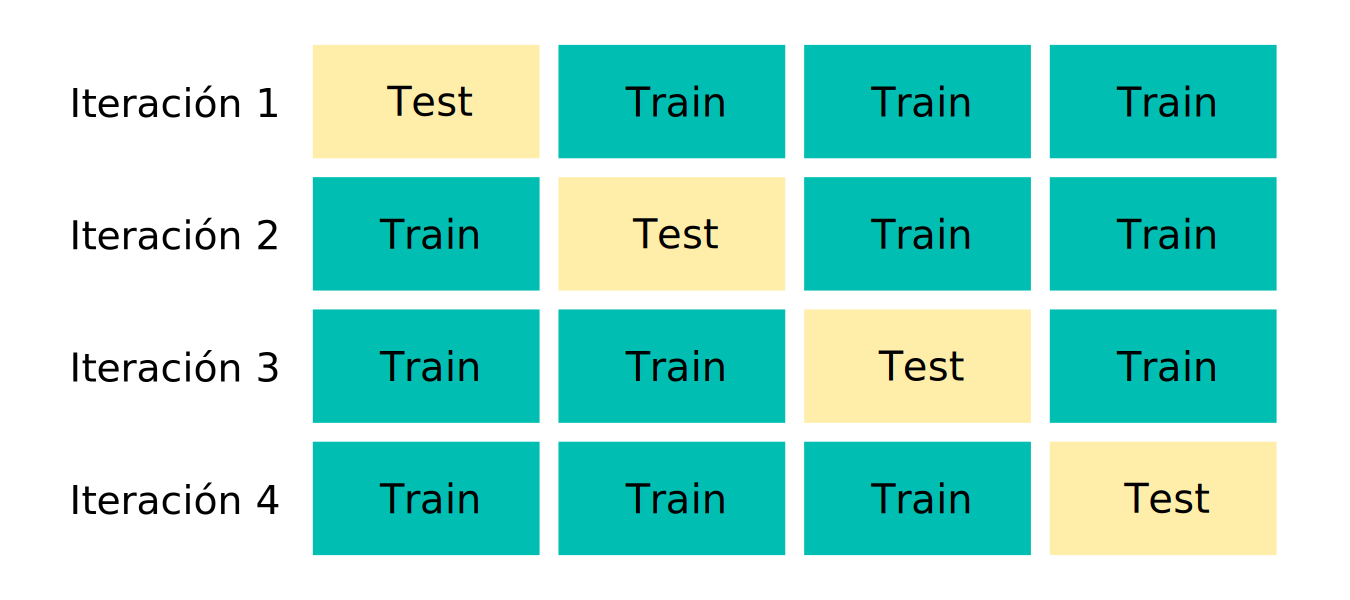
\includegraphics[width=10cm]{figs/KFold_explanation.png}
  \end{center}
  \captionsetup{justification=centering}
  \caption{Ejemplo de división de la base de datos \\
  en 4 \textit{pliegues} usando KFold.}
  \label{fig:kfolf_explicacion}
\end{figure}

La clase con menos datos del dataset, tiene una cantidad de 28. Por lo tanto, se usan 4 \textit{pliegues} para KFold, de esta manera aseguramos 7 datos de esa clase en cada pliegue. Al tener una base de datos desequilibrada, esto es, que no tiene el mismo número de muestras para todas las clases, debemos usar KFold Stratified, que nos asegura poseer siempre el mismo porcentaje de muestras de cada clase en todos los pliegues.\\

KFold Stratified por lo tanto, nos sirve para encontrar los parámetros óptimos de cada algoritmo. Por ejemplo, para KNN probamos cada una de las \textit{k} (vecinos) posibles en cada una de las iteraciones. El resultado es una matriz con el \textit{Accuracy} para cada una de las \textit{k} en cada una de las iteraciones. Finalmente, se calcula la media de todas las iteraciones y se escoge la \textit{k} que más \textit{Accuracy} de media haya obtenido. Y así conseguimos el número de vecinos óptimo. Un ejemplo con 4 valores de vecinos se muestra en la Figura \ref{fig:kfold_KNN}.\\

\begin{figure} [h!]
  \begin{center}
    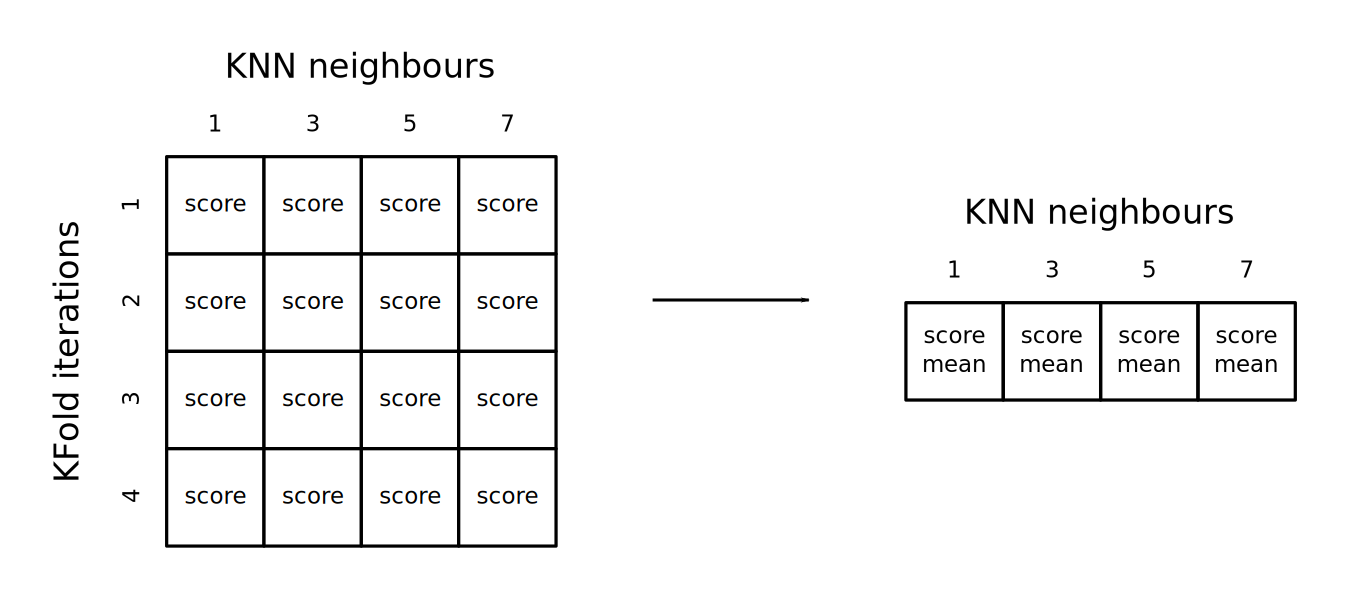
\includegraphics[width=13cm]{figs/KFold_KNN.png}
  \end{center}
  \captionsetup{justification=centering}
  \caption{Ejemplo de búsqueda del número de vecinos\\
  óptimo para KNN usando KFold.}
  \label{fig:kfold_KNN}
\end{figure}

Sin embargo, como se usa PCA para reducir el número de características (componentes), debemos encontrar además el número óptimo de las mismas. Entonces, en vez de tener una matriz de 2 dimensiones, pasamos a trabajar con una matriz de 3 dimensiones. Se puede ver un ejemplo en la Figura \ref{fig:kfold_KNN_PCA}. Al igual que en el caso anterior, la combinación óptima de vecinos y componentes de PCA, es la que haya obtenido mejor puntuación de media.\\

\begin{figure} [h!]
  \begin{center}
    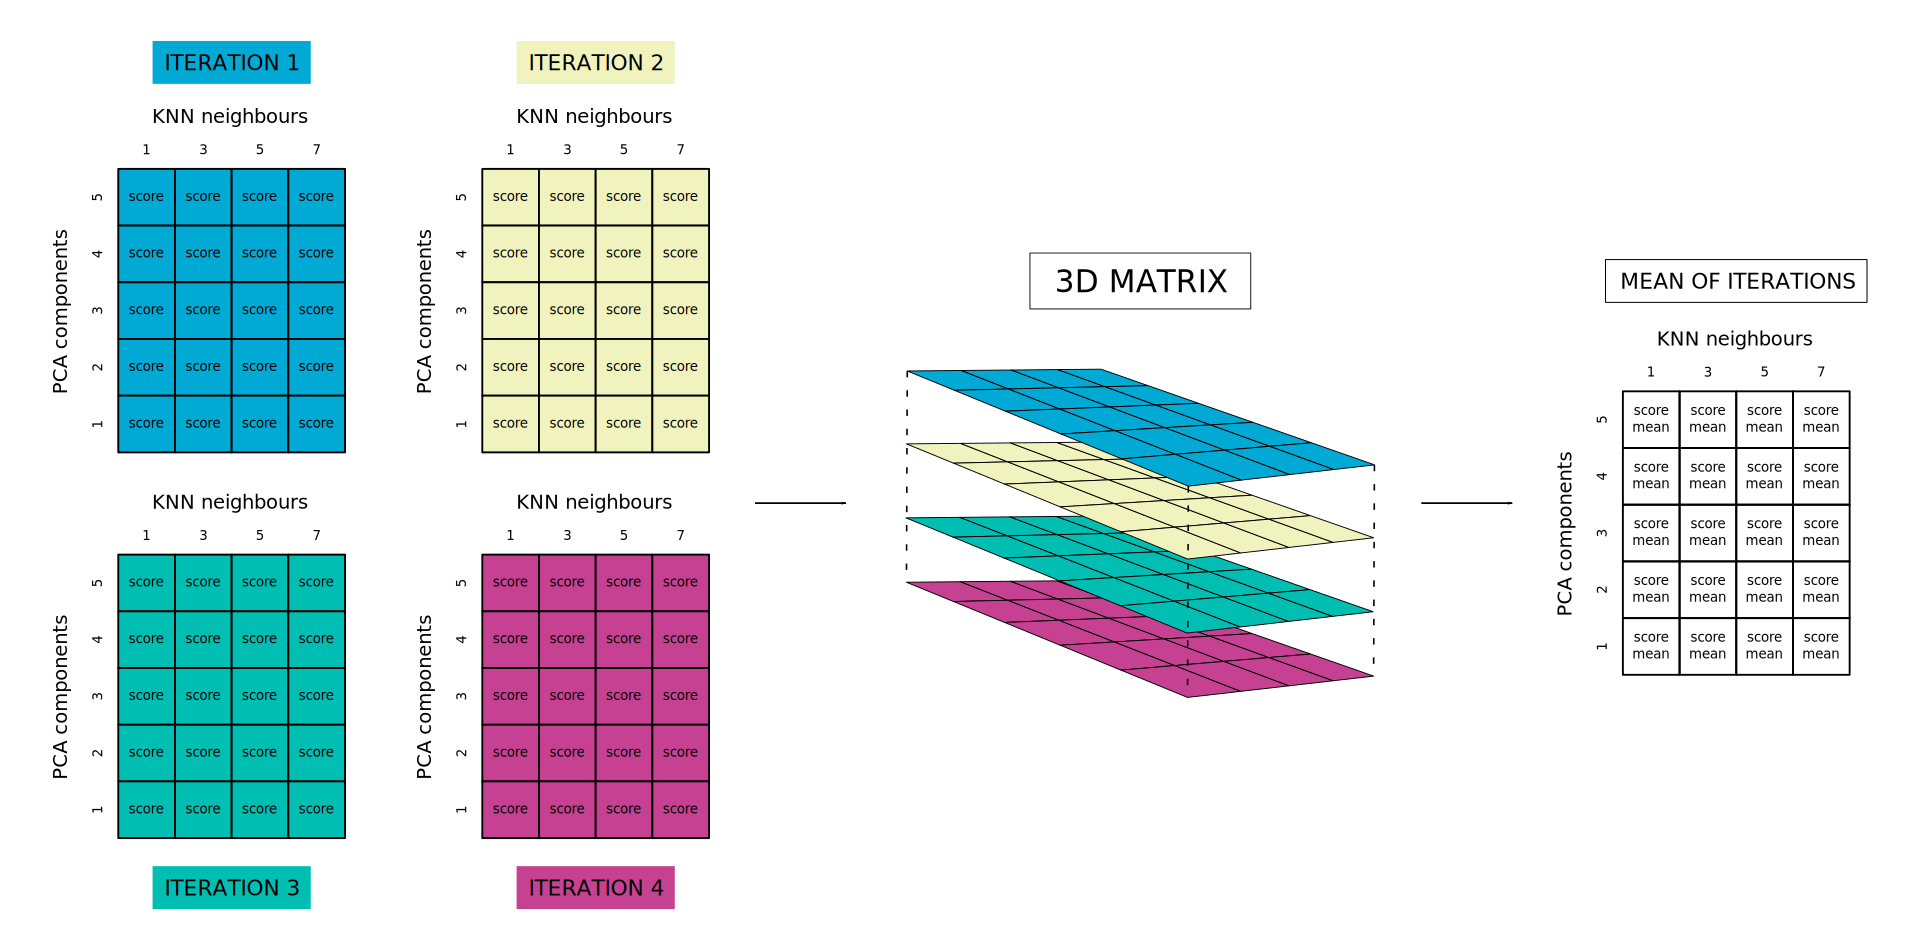
\includegraphics[width=16cm]{figs/KFold_KNN_PCA.png}
  \end{center}
  \captionsetup{justification=centering}
  \caption{Ejemplo de búsqueda del número de vecinos\\
  óptimo para KNN y el número de componentes\\
  óptimo a reducir por PCA usando KFold.}
  \label{fig:kfold_KNN_PCA}
\end{figure}

En este trabajo, el valor óptimo de características a mantener por PCA y los parámetros óptimos para cada clasificador tras realizar su búsqueda usando validación cruzada KFoldStratified de 4 \textit{pliegues}, se encuentran en el Cuadro \ref{cuadro:parametros_optimos}. Para hacer la reducción con PCA, se ha probado con un número de componentes entre 2 y 20 incluidos, para KNN se ha probado con valores de k impares entre 1 y 13 incluidos, para SVM con valores de C entre 1 y 999 (saltos de 10 en 10) y para MLP se ha probado con 1 capa oculta de neuronas entre 5 y 24 incluidos, no ha sido necesario añadir más capas.\\

\begin{table}[H]
\begin{center}
\begin{tabular}{|c|c|}
     \hline
    \textbf{Clasificador y PCA} & \textbf{Parámetros} \\
    \hline
     KNN y PCA & \verb|k = 7|, \verb|n_components = 11|\\
     SVM y PCA & \verb|C = 21|, \verb|n_components = 11|\\
     MLP y PCA & \verb|hidden_layer_sizes = (17)|, \verb|n_components = 11|\\
     \hline
 \end{tabular}
 \captionsetup{justification=centering}
\caption{Parámetros óptimos para cada uno de los clasificadores y PCA.}
\label{cuadro:parametros_optimos}
\end{center}
\end{table}

Finalmente, los resultados obtenidos en el entrenamiento usando los parámetros óptimos, se encuentran en el Cuadro \ref{cuadro:resultados}. Estos resultados de precisión han sido calculados también mediante validación cruzada KFoldStratified de 4 \textit{pliegues}, y se muestra la media de todas las iteraciones.\\

\begin{table}[H]
\begin{center}
\begin{tabular}{|c|c|c|c|c|}
     \hline
    \textbf{Clasificador} & \textbf{Accuracy} & \textbf{Precision} & \textbf{Recall} & \textbf{F1-score}\\
    \hline
     KNN & 0.95 & 0.93 & 0.94 & 0.92\\
     SVM & 0.95 & 0.93 & 0.92 & 0.92\\
     MLP & 0.95 & 0.95 & 0.93 & 0.93\\
     \hline
 \end{tabular}
 \captionsetup{justification=centering}
\caption{Resultados de precisión de los clasificadores en el entrenamiento.}
\label{cuadro:resultados}
\end{center}
\end{table}

Como conclusiones finales, observamos que hemos obtenido unos resultados muy buenos para los tres clasificadores, con un porcentaje de acierto medio del 95\%. Además, consultando por separado los resultados de cada una de las clases en cada una de las iteraciones de la validación cruzada, afirmamos también que ninguna emoción de forma individual tiene malos resultados. Por ejemplo, para el entrenamiento con KNN (Cuadro \ref{cuadro:resultados_KNN_emociones}).\\

\begin{table}[h]
\begin{minipage}{0.48\linewidth}
\centering
\begin{adjustbox}{max width=\textwidth}
\begin{tabular}{|c|c|c|c|}
\hline
\textbf{Clase} & \textbf{Precision} & \textbf{Recall} & \textbf{F1-score}\\
\hline
     Enfado & 0.88 & 0.58 & 0.70\\
     Felicidad & 0.94 & 1.00 & 0.97\\
     Tristeza & 0.58 & 1.00 & 0.74\\
     Sorpresa & 1.00 & 0.90 & 0.95\\
\hline
\end{tabular}
\end{adjustbox}
\vspace{0.5cm}

\begin{adjustbox}{max width=\textwidth}
\begin{tabular}{|c|c|c|c|}
\hline
\textbf{Clase} & \textbf{Precision} & \textbf{Recall} & \textbf{F1-score}\\
\hline
     Enfado & 1.00 & 1.00 & 1.00\\
     Felicidad & 1.00 & 1.00 & 1.00\\
     Tristeza & 1.00 & 1.00 & 1.00\\
     Sorpresa & 1.00 & 1.00 & 1.00\\
\hline
\end{tabular}
\end{adjustbox}
\end{minipage}\hfill
\begin{minipage}{0.48\linewidth}
\centering
\begin{adjustbox}{max width=\textwidth}
\begin{tabular}{|c|c|c|c|}
\hline
\textbf{Clase} & \textbf{Precision} & \textbf{Recall} & \textbf{F1-score}\\
\hline
     Enfado & 1.00 & 0.82 & 0.90\\
     Felicidad & 1.00 & 1.00 & 1.00\\
     Tristeza & 0.78 & 1.00 & 0.88\\
     Sorpresa & 1.00 & 1.00 & 1.00\\
\hline
\end{tabular}
\end{adjustbox}
\vspace{0.5cm}

\begin{adjustbox}{max width=\textwidth}
\begin{tabular}{|c|c|c|c|}
\hline
\textbf{Clase} & \textbf{Precision} & \textbf{Recall} & \textbf{F1-score}\\
\hline
     Enfado & 0.90 & 0.82 & 0.86\\
     Felicidad & 1.00 & 1.00 & 1.00\\
     Tristeza & 0.75 & 0.86 & 0.80\\
     Sorpresa & 1.00 & 1.00 & 1.00\\
\hline
\end{tabular}
\end{adjustbox}
\end{minipage}
\captionsetup{justification=centering}
\caption{Resultados del entrenamiento con KNN en cada una\\
de las 4 iteraciones de KFoldStratified}
\label{cuadro:resultados_KNN_emociones}
\end{table}

Los modelos entrenados son guardados en ficheros con formato \textit{pkl} usando el módulo \textit{pickle} de Python. De esta manera, pueden ser cargados en cualquier otro programa y realizar predicciones con ellos usando el método \verb|predict()|. A este último se le introducen los ángulos del rostro a clasificar y este devuelve la clase predicha.\\

\section{Integración del sistema en ROS}
\label{sec:integración_en_ros}

El último paso a llevar a cabo en este trabajo es integrar el sistema de detección de emociones en ROS para facilitar su uso en un sistema robótico. Con esto, se pretende crear una herramienta que abstraiga al desarrollador del código del sistema y, que por lo tanto, a través de \textit{topics} de ROS se puedan obtener todos los datos detectados por el sistema de manera fácil.\\

En esta sección se comenzará explicando cuál ha sido el proceso llevado a cabo para instalar ROS bajo Raspberry Pi OS, se comentará la estructura del paquete y del código ROS desarrollado y, por último, se hará una explicación de su funcionamiento, comentando aspectos de su rendimiento.

\subsection{Instalación de ROS en Raspberry}

El objetivo principal es instalar ROS2, pero no existe ninguna versión de este compatible con 32-bit, y la reciente versión de 64-bit de Raspberry Pi OS lanzada por primera vez en enero de este año, a fecha de hoy, no tiene total compatibilidad con todas las librerías usadas en este trabajo. Igualmente, se ha intentado instalar ROS2 en Raspberry Pi OS de 64-bit, pero no ha resultado satisfactorio porque hay paquetes que no son compatibles con un procesador ARM.\\

Finalmente, se instaló ROS Noetic, ya que existe una versión del mismo para Debian Buster, y la versión de Raspberry Pi OS usada en este trabajo está basada en Debian Buster. Sin embargo, no se puede hacer la instalación de la forma tradicional a través de \textit{apt}, porque dicha versión de ROS tiene soporte nivel 3 \footnote{Nivel 3: no existen archivos binarios, el usuario debe compilar el código desde la fuente}. Los pasos a seguir para su instalación son los siguientes\footnote{\url{https://varhowto.com/install-ros-noetic-raspberry-pi-4/}}:

\begin{enumerate}
\item Añadimos el repositorio oficial de ROS para Debian.
\begin{listing}[style=consola, numbers=none]
$ sudo sh -c 'echo "deb http://packages.ros.org/ros/ubuntu buster main" > /etc/apt/sources.list.d/ros-noetic.list'
\end{listing}

\item Agregamos la clave de ROS para asegurarnos de que instalamos paquetes de ROS autenticados.
\begin{listing}[style=consola, numbers=none]
$ sudo apt-key adv --keyserver 'hkp://keyserver.ubuntu.com:80' --recv-key C1CF6E31E6BADE8868B172B4F42ED6FBAB17C654
\end{listing}

\item Actualizamos los repositorios del sistema.
\begin{listing}[style=consola, numbers=none]
$ sudo apt-get update
\end{listing}

\item Instalamos las dependencias de compilación.
\begin{listing}[style=consola, numbers=none]
$ sudo apt-get install -y python-rosdep python-rosinstall-generator python-wstool python-rosinstall build-essential cmake
\end{listing}

\item Inicializamos \verb|rosdep|.
\begin{listing}[style=consola, numbers=none]
$ sudo rosdep init
$ rosdep update
\end{listing}

\item Creamos un espacio de trabajo de ROS.
\begin{listing}[style=consola, numbers=none]
$ mkdir ~/ros_catkin_ws 
$ cd ~/ros_catkin_ws
\end{listing}

\item Usamos \verb|rosinstall_generator| para generar una lista de dependencias de Noetic para la variante \verb|ros_comm|, porque los tradicionales \verb|desktop-full| o \verb|desktop| no son compatibles y la placa Raspberry no posee la suficiente memoria como para compilar rviz.
\begin{listing}[style=consola, numbers=none]
$ rosinstall_generator ros_comm --rosdistro noetic --deps --wet-only --tar > noetic-ros_comm-wet.rosinstall
\end{listing}

\item Usamos \verb|wstool| para obtener todos los repositorios.
\begin{listing}[style=consola, numbers=none]
$ wstool init src noetic-ros_comm-wet.rosinstall
\end{listing}

\item Instalamos dependencias usando \verb|rosdep|.
\begin{listing}[style=consola, numbers=none]
$ rosdep install -y --from-paths src --ignore-src --rosdistro noetic -r --os=debian:buster
\end{listing}

\item Por último, antes de compilar, aumentamos el espacio de \verb|swap| que se usará cuando se agote la memoria física en la Raspberry. Primero desactivamos la memoria \verb|swap|.
\begin{listing}[style=consola, numbers=none]
$ sudo dphys-swapfile swapoff
\end{listing}

\item Editamos el archivo \verb|/etc/dphys-swapfile|, cambiando \verb|CONF_SWAPSIZE=100| por \verb|CONF_SWAPSIZE=1024|. Y volvemos a configurar y activar la \verb|swap|.
\begin{listing}[style=consola, numbers=none]
$ sudo dphys-swapfile setup
$ sudo dphys-swapfile swapon
\end{listing}

\item Procedemos a realizar la compilación, todo se instalará en \verb|/opt/ros/noetic|.
\begin{listing}[style=consola, numbers=none]
$ sudo src/catkin/bin/catkin_make_isolated --install -DCMAKE_BUILD_TYPE=Release --install-space /opt/ros/noetic -j1 -DPYTHON_EXECUTABLE=/usr/bin/python3
\end{listing}
\end{enumerate}

\subsection{Estructura ROS y código desarrollado}

Se ha desarrollado un paquete llamado \verb|emotion_detection_ros|\footnote{\url{https://github.com/jmrtzma/emotion_detection_ros}}, cuyo esquema general de funcionamiento se puede ver en la Figura \ref{fig:esquema_paquete_ROS}.\\

\begin{figure} [h!]
  \begin{center}
    \includegraphics[width=15cm]{figs/paquete_ros.png}
  \end{center}
  \captionsetup{justification=centering}
  \caption{Esquema general del paquete de ROS.}
  \label{fig:esquema_paquete_ROS}
\end{figure}

El nodo \verb|emotion_detection| recibe los \textit{frames} de una cámara a través de un \textit{topic} que maneja mensajes del tipo \verb|sensor_msgs/CompressedImage|. Este nodo se encargará de hacer todo el procesamiento, y a través de otro \textit{topic} que maneja mensajes del tipo \verb|emotion_detection_ros_msgs/BoundingBoxes|, envía una lista de \verb|emotion_detection_ros_msgs/BoundingBox|. Cada uno de estos últimos mensajes contiene la información de cada emoción detectada: un valor tipo \textit{float64} con la probabilidad de la predicción, cuatro campos de tipo \textit{int64} con las coordenadas del bounding box que rodea la emoción detectada, y un \textit{string} con la emoción detectada.

\subsubsection{Parámetros de configuración}

El paquete posee un directorio \textit{config} en el que se encuentran dos ficheros de configuración. Estos son de formato \textit{yaml}, y sirven para personalizar parámetros del código sin necesidad de editar el mismo.\\

El fichero \verb|model.yaml| (Código \ref{cod:model}) nos permite cambiar el algoritmo que usará nuestro sistema para realizar la clasificación de emociones (KNN, SVM o MLP) y elegir el número máximo de caras que deseamos que se detecten. Este último nos permite controlar el rendimiento ofrecido, ya que por cada cara nueva que se esté detectando, los FPS se reducen.\\

\begin{code}[h]
\begin{lstlisting}
model:

  algorithm: KNN
  max_num_faces: 1
\end{lstlisting}
\captionsetup{justification=centering}
\caption[Fichero de configuración model.yaml.]{Fichero de configuración model.yaml.}
\label{cod:model}
\end{code}

El fichero \verb|ros.yaml| (Código \ref{cod:ros_yaml}) nos permite cambiar los nombres de los \textit{topics} usados, además de algunos parámetros de configuración de los publicadores y suscriptores. Por último, podemos elegir si deseamos que se muestre el visualizador o no, así como el delay entre los \textit{frames} mostrados en este.

\begin{code}[h]
\begin{lstlisting}
subscribers:

  camera_reading:
    topic: /raspicam_node/image/compressed
    queue_size: 1

publishers:

  bounding_boxes:
      topic: /emotion_detection_ros/bounding_boxes
      queue_size: 1
      latch: False

image_view:

  enable: True
  wait_key_delay: 1
\end{lstlisting}
\captionsetup{justification=centering}
\caption[Fichero de configuración ros.yaml.]{Fichero de configuración ros.yaml.}
\label{cod:ros_yaml}
\end{code}

\subsubsection{Ficheros de código}

El nodo principal se encuentra en el fichero \verb|emotion_detection_node.py| del directorio \verb|scripts|. Este posee dos \textit{threads}. El principal del programa se encarga de recibir los \textit{frames} a través de un subscriptor, y el otro \textit{thread} se encarga de realizar el procesamiento de los frames, esto es: realizar las predicciones, dibujar el bounding box, dibujar el valor de FPS y, además, publicar los datos obtenidos en el \textit{topic} correspondiente. Se ha organizado de esta manera para conseguir un mayor rendimiento ya que, realizando el procesamiento en un \textit{thread} distinto al principal, no se tratarán estrictamente todos los frames, lo que impulsará considerablemente el valor de FPS del sistema.\\

Las tareas del nodo principal están repartidas en diferentes clases que se encuentran en el directorio \verb|src|:

\begin{itemize}
    \item \verb|EmotionalMesh|. Encapsula cada \textit{malla emocional} detectada. Recibe como entrada las coordenadas de los puntos faciales detectados por MediaPipe FaceMesh y, con ello, forma la \textit{malla emocional} y calcula todos los ángulos.
    
    \item \verb|EmotionalMeshDetection|. Se encarga de detectar los puntos faciales de la cara usando MediaPipe FaceMesh y, con ello, genera una lista de objetos \verb|EmotionalMesh|, esto es, una lista con las \textit{mallas emocionales} de las caras detectadas en el \textit{frame}.
    
    \item \verb|Emotion|. Encapsula los datos de cada predicción realizada, esto es, el nombre de la emoción, la probabilidad, la etiqueta que se mostrará por pantalla que contiene el nombre de la emoción y la probabilidad, y las coordenadas del bounding box que rodea esa cara.
    
    \item \verb|EmotionPredictor|. Se encarga de realizar las predicciones en los frames usando el modelo entrenado y los objetos \verb|EmotionalMesh|. Genera una lista de objetos \verb|Emotion| con los datos de las predicciones.
\end{itemize}

\subsection{Uso y rendimiento}
\label{sec:uso_rendimiento_ros}

Gracias a que el sistema está integrado en ROS y la comunicación se produce a través de \textit{topics}, se podría usar cualquier cámara que publique \textit{frames} en el \textit{topic} necesario. Sin embargo, se recomienda usar la Raspberry Pi Camera V2.1, ya que ha sido la cámara usada en este trabajo.\\

Para usar dicha cámara en nuestro entorno ROS, se ha hecho uso del paquete \verb|raspicam_node| \footnote{\url{https://github.com/UbiquityRobotics/raspicam_node}}. Este se encarga de leer \textit{frames} de la Raspberry Pi Camera de forma eficiente y publicarlos en el \textit{topic} \verb|/raspicam_node/image/compressed|.\\

Con los paquetes \verb|emotion_detection_ros| y \verb|raspicam_node| compilados en el \textit{workspace} de ROS, los pasos a seguir para poner en marcha el sistema son los siguientes:

\begin{enumerate}
\item Lanzamos el launcher de la cámara.
\begin{listing}[style=consola, numbers=none]
$ roslaunch raspicam_node camerav2_410x308_30fps.launch
\end{listing}

\item Lanzamos el sistema de detección de emociones
\begin{listing}[style=consola, numbers=none]
$ roslaunch emotion_detection_ros emotion_detection_ros.launch
\end{listing}
\end{enumerate}

Tras lanzar el sistema, se abrirá una ventana gráfica en la que se mostrarán los \textit{frames}, en los cuales aparecerán dibujados los bounding boxes con sus respectivas etiquetas mostrando la predicción (Figura \ref{fig:ventana_grafica_1_cara}). Además, en la esquina superior izquierda se expondrá el valor de FPS del sistema.\\

\begin{figure}[h!]
  \begin{center}
  \subcapcentertrue
    \subfigure[Predicción de felicidad]{\includegraphics[width=75mm]{figs/prediccion_happy.png}}
    \subfigure[Predicción de enfado]{\includegraphics[width=75mm]{figs/prediccion_anger.png}}
    \subfigure[Predicción de tristeza]{\includegraphics[width=75mm]{figs/prediccion_sadness.png}}
    \subfigure[Predicción de sorpresa]{\includegraphics[width=75mm]{figs/prediccion_surprise.png}}
  \end{center}
 \captionsetup{justification=centering}
\caption{Ejemplos de la ventana gráfica del sistema de detección\\
de emociones funcionando en ROS.}
\label{fig:ventana_grafica_1_cara}
\end{figure}

Otro ejemplo, esta vez detectando dos caras, se encuentra en la Figura \ref{fig:ventana_grafica_2_caras}. Y si ejecutamos el comando \verb|rostopic echo /emotion_detection_ros/bounding_boxes|, podemos observar cómo la información detectada se está publicando en dicho \textit{topic} (Código \ref{cod:ejemplo_salida_topic}).\\

\begin{figure} [h!]
  \begin{center}
    \includegraphics[width=75mm]{figs/prediccion_happy_surprise.png}
  \end{center}
  \captionsetup{justification=centering}
  \caption{Ejemplo del sistema en ROS detectando las\\
  emociones de dos caras.}
  \label{fig:ventana_grafica_2_caras}
\end{figure}

\begin{code}[h]
\begin{listing}[style=consola, numbers=none]
---
bounding_boxes:
    -
        probability: 100.0
        xmin: 198
        ymin: 199
        xmax: 234
        ymax: 249
        Class: "Surprise"
    -
        probability: 100.0
        xmin: 42
        ymin: 74
        xmax: 131
        ymax: 177
        Class: "Happy"
---
\end{listing}
\captionsetup{justification=centering}
\caption[Información publicada en el \textit{topic} /emotion\_detection\_ros/bounding\_boxes para el ejemplo de la Figura \ref{fig:ventana_grafica_2_caras}.]{Ejemplo de información publicada en el \textit{topic} /emotion\_detection\_ros/bounding\_boxes para el ejemplo de la Figura \ref{fig:ventana_grafica_2_caras}.}
\label{cod:ejemplo_salida_topic}
\end{code}

En cuanto al rendimiento general del sistema, se ha realizado un estudio del valor de FPS arrojado dependiendo del número de caras detectadas. Se han realizado tres pruebas, en cada una de ellas modificando el parámetro de configuración \verb|max_num_faces| del fichero \verb|model.yaml|. De esta manera se ha probado el sistema con hasta tres caras. Los resultados de las tres situaciones se encuentran en los Cuadros \ref{cuadro:rendimiento_ros_1}, \ref{cuadro:rendimiento_ros_2} y \ref{cuadro:rendimiento_ros_3}, respectivamente.\\

\begin{table}[H]
\begin{center}
\begin{adjustbox}{max width=\textwidth}
\begin{tabular}{|c|c|c|c|}
     \hline
    \textbf{Caras detectadas} & \textbf{Media de FPS} & \textbf{Valor máximo de FPS} & \textbf{Valor mínimo de FPS}\\
    \hline
     1 & 13.18 & 15.13 & 11.04\\
     \hline
 \end{tabular}
 \end{adjustbox}
 \captionsetup{justification=centering}
\caption{Rendimiento del sistema en ROS con max\_num\_faces: 1.}
\label{cuadro:rendimiento_ros_1}
\end{center}
\end{table}

\begin{table}[H]
\begin{center}
\begin{adjustbox}{max width=\textwidth}
\begin{tabular}{|c|c|c|c|}
     \hline
    \textbf{Caras detectadas} & \textbf{Media de FPS} & \textbf{Valor máximo de FPS} & \textbf{Valor mínimo de FPS}\\
    \hline
     1 & 11.11 & 11.97 & 9.18\\
     2 & 7.53 & 8.35 & 6.96\\
     \hline
 \end{tabular}
 \end{adjustbox}
 \captionsetup{justification=centering}
\caption{Rendimiento del sistema en ROS con max\_num\_faces: 2.}
\label{cuadro:rendimiento_ros_2}
\end{center}
\end{table}

\begin{table}[H]
\begin{center}
\begin{adjustbox}{max width=\textwidth}
\begin{tabular}{|c|c|c|c|}
     \hline
    \textbf{Caras detectadas} & \textbf{Media de FPS} & \textbf{Valor máximo de FPS} & \textbf{Valor mínimo de FPS}\\
    \hline
     1 & 11.05 & 11.72 & 9.41\\
     2 & 6.77 & 7.61 & 6.15\\
     3 & 5.37 & 6.93 & 5.02\\
     \hline
 \end{tabular}
 \end{adjustbox}
 \captionsetup{justification=centering}
\caption{Rendimiento del sistema en ROS con max\_num\_faces: 3.}
\label{cuadro:rendimiento_ros_3}
\end{center}
\end{table}